\documentclass[12pt,]{article}
\usepackage{lmodern}
\usepackage{amssymb,amsmath}
\usepackage{ifxetex,ifluatex}
\usepackage{fixltx2e} % provides \textsubscript
\ifnum 0\ifxetex 1\fi\ifluatex 1\fi=0 % if pdftex
  \usepackage[T1]{fontenc}
  \usepackage[utf8]{inputenc}
\else % if luatex or xelatex
  \ifxetex
    \usepackage{mathspec}
  \else
    \usepackage{fontspec}
  \fi
  \defaultfontfeatures{Ligatures=TeX,Scale=MatchLowercase}
\fi
% use upquote if available, for straight quotes in verbatim environments
\IfFileExists{upquote.sty}{\usepackage{upquote}}{}
% use microtype if available
\IfFileExists{microtype.sty}{%
\usepackage{microtype}
\UseMicrotypeSet[protrusion]{basicmath} % disable protrusion for tt fonts
}{}
\usepackage[left=1in, right=1in, top=1in, bottom=1in, headheight=12pt, letterpaper]{geometry}
\usepackage{hyperref}
\hypersetup{unicode=true,
            pdftitle={A simulation-based approach for quantifying and partitioning uncertainty to improve ecological forecasts},
            pdfauthor={Andrew T. Tredennick\^{}\{1\}, Peter B. Adler\^{}1, and others\^{}\{2\}},
            pdfborder={0 0 0},
            breaklinks=true}
\urlstyle{same}  % don't use monospace font for urls
\usepackage{graphicx,grffile}
\makeatletter
\def\maxwidth{\ifdim\Gin@nat@width>\linewidth\linewidth\else\Gin@nat@width\fi}
\def\maxheight{\ifdim\Gin@nat@height>\textheight\textheight\else\Gin@nat@height\fi}
\makeatother
% Scale images if necessary, so that they will not overflow the page
% margins by default, and it is still possible to overwrite the defaults
% using explicit options in \includegraphics[width, height, ...]{}
\setkeys{Gin}{width=\maxwidth,height=\maxheight,keepaspectratio}
\IfFileExists{parskip.sty}{%
\usepackage{parskip}
}{% else
\setlength{\parindent}{0pt}
\setlength{\parskip}{6pt plus 2pt minus 1pt}
}
\setlength{\emergencystretch}{3em}  % prevent overfull lines
\providecommand{\tightlist}{%
  \setlength{\itemsep}{0pt}\setlength{\parskip}{0pt}}
\setcounter{secnumdepth}{0}
% Redefines (sub)paragraphs to behave more like sections
\ifx\paragraph\undefined\else
\let\oldparagraph\paragraph
\renewcommand{\paragraph}[1]{\oldparagraph{#1}\mbox{}}
\fi
\ifx\subparagraph\undefined\else
\let\oldsubparagraph\subparagraph
\renewcommand{\subparagraph}[1]{\oldsubparagraph{#1}\mbox{}}
\fi

%%% Use protect on footnotes to avoid problems with footnotes in titles
\let\rmarkdownfootnote\footnote%
\def\footnote{\protect\rmarkdownfootnote}

%%% Change title format to be more compact
\usepackage{titling}

% Create subtitle command for use in maketitle
\newcommand{\subtitle}[1]{
  \posttitle{
    \begin{center}\large#1\end{center}
    }
}

\setlength{\droptitle}{-2em}
  \title{A simulation-based approach for quantifying and partitioning uncertainty
to improve ecological forecasts}
  \pretitle{\vspace{\droptitle}\centering\huge}
  \posttitle{\par}
  \author{Andrew T. Tredennick\(^{1}\), Peter B. Adler\(^1\), and others\(^{2}\)}
  \preauthor{\centering\large\emph}
  \postauthor{\par}
  \date{}
  \predate{}\postdate{}

\usepackage{mathptmx}
\usepackage{upgreek}
\usepackage{bm}
\usepackage{setspace}
\usepackage{booktabs}
\doublespacing
\usepackage{lineno}
\linenumbers

\begin{document}
\maketitle

\setlength{\abovedisplayskip}{0pt}\raggedright

\(^1\) Department of Wildland Resources and the Ecology Center, Utah
State University, Logan, UT, United States

\(^2\) Department of somewhere

\hypertarget{abstract}{%
\section{Abstract}\label{abstract}}

Making informed ecosystem management decisions in the face of rapid
environmental change requires forecasts from models of ecological
processes. However, forecasts from ecological models are often
associated with high degrees of uncertainty, making it difficult for
such forecasts to inform decision-making processes. To make progress
toward the goal of reliable and informative ecological forecasts, we
need to know from where forecast uncertainty arises. Such knowledge can
guide investment in future research that will most improve forecast
skill. There is a rich history of analytical expressions that partition
the variance of future dynamics, but these expressions suffer from
necessary assumptions such as linear dynamics and small-variance
approximations that exclude interactions. Similarly, the earth systems
modeling community has developed methods for paritioning uncertainty of
model projections, but these operate at a different modeling grain than
most of ecology. Building on these approaches, we develop a
simulation-based approach for quantifying and partitioning forecast
uncertainty from Bayesian state-space models that overcomes the
limitations of previous analytical approaches. Our approach is similar
to an Analysis of Variance, where the total variance of a forecast is
paritioned among its constituent parts, namely initial conditions
uncertainty, parameter uncertainty, driver uncertainty, process error,
and their interactions. We demonstrate the approach with simulated data
and with an empirical example using data from the Yellowstone bison
population. We also provide functions written in the statistical
programming language R, which will allow others using Bayesian
state-space models to employ our approach in their own research.

\emph{Keywords: Bayesian state-space model, forecast, Markov chain Monte
Carlo, prediction, population model, uncertainty, Yellowstone bison}

\hypertarget{introduction}{%
\section{Introduction}\label{introduction}}

A fundamental challenge facing society is to predict the ecological
impacts of global environmental changes such as nitrogen deposition,
climate change, and habitat fragmentation. Each of these global change
drivers have now exceeded their historical ranges of variability
(Steffen et al. 2015), ushering in a no-analog era in which the past
cannot predict the future. We can, however, look to the past to
parameterize models that allow us to forecast the future states of
ecological systems (Clark et al. 2001, Dietze et al. 2018). Ecologists
are in an excellent position to meet this forecasting challenge because
we have spent decades gaining understanding of the processes that
regulate populations, communities, and ecosystems. However, we lack a
systematic understanding of the current limits to ecological forecasts.
As a result, we do not know how to allocate research effort to improve
our forecasts.

Making poor forecasts is inevitable as ecology matures into a more
predictive science. The key is to learn from our failures so that
forecasts become more accurate over time. The success of meteorological
forecasting tells us that basic research on the causes of forecast
uncertainty is an essential component of this learning process (Bauer et
al. 2015).

Various approaches have been used to characterize and partition forecast
uncertainty (Sobol' 1993, Cariboni et al. 2007). For example, consider a
dynamic model designed to predict some state \emph{y} in the future
(\(y_{t+1}\)) based on the current state (\(y_{t}\)), an environmental
driver(s) (\(x\)), parameters (\(\theta\)), and process error
(\(\epsilon\)). We can then write a general form of the model as:

\begin{align}
y_{t+1} = f(y_t, x_t|\theta) + \epsilon_{t+1},
\end{align}

which states that \(y\) at time \(t+1\) is a function of \(y\) and \(x\)
at time \(t\) conditional on the model parameters (\(\theta\)) plus
process error (\(\epsilon\)). Ignoring covariance among factors and
assuming linear dynamics, Dietze (2017), following Sobol' (1993) and
Cariboni et al. (2007), suggests that forecast variance
(\(Var[y_{t+1}]\)) is approximately:

\begin{align}
Var[y_{t+1}] \approx \underbrace{\left(\frac{\delta f}{\delta y} \right)^2}_{\text{stability}} 
               \underbrace{\vphantom{ \left(\frac{\delta f}{\delta y} \right)^2 } Var[y_t]}_{\text{IC uncert.}} +
               \underbrace{\vphantom{ \left(\frac{\delta f}{\delta y} \right)^2 }\left(\frac{\delta f}{\delta x} \right)^2}_{\text{driver sens.}} 
               \underbrace{\vphantom{ \left(\frac{\delta f}{\delta y} \right)^2 } Var[x_t]}_{\text{driver uncert.}} +
               \underbrace{\vphantom{ \left(\frac{\delta f}{\delta y} \right)^2 }\left(\frac{\delta f}{\delta \theta} \right)^2}_{\text{param sens.}}
               \underbrace{\vphantom{ \left(\frac{\delta f}{\delta y} \right)^2 } Var[\theta]}_{\text{param. uncert.}} +
               \underbrace{\vphantom{ \left(\frac{\delta f}{\delta y} \right)^2 } Var[\epsilon_{t+1}]}_{\text{process error}},
\end{align}

where each additive term follows a pattern of \emph{sensitivity} times
\emph{variance} and ``IC uncert.'' refers to ``\emph{I}nitial
\emph{C}onditions uncertainty.'' The variance attributable to any
particular factor is a function of how sensitive the model is to the
factor and the variance of that factor. For example, the atmosphere is a
chaotic system, meaning its dynamics are internally unstable and
sensitive to initial conditions uncertainty. This is why billions of
dollars are spent each year to measure meterological variables --
meterologists learned that the key to reducing forecast error
\((Var[y_{t+1}])\) was to reduce the uncertainty of initial conditions
(\(Var[y_t]\)). In contrast, ecologists are attempting to make
actionable forecasts with little knowledge of which term in Eq. 2
dominates forecast error. Knowing which term dominates forecast error in
different ecological settings will advance our fundamental understanding
of the natural world and immediately impact practical efforts to
monitor, model, and predict ecological dynamics.

While having an analytical expression such as Eq. 2 is satisfying,
arriving at the expression involves strict assumptions. First, Eq. 2
only holds when the underlying dynamics are linear, which may not be the
case for many populations and models. Second, Eq. 2 only includes
additive effects of each factor because the Taylor series decomposition
requires small-variance approximations that eliminate interactions. But,
interactions among the factors are probably commone. For example, in a
simple simulation of an AR(1) process, we show that initial conditions
uncertainty and parameter error interact to generate the full spread of
forecast variance (Figure 1). Therefore, progress in quantifying and
partioning forecast uncertainty requires a more flexible approach than
that provided by Eq. 2.

\begin{figure}
\centering
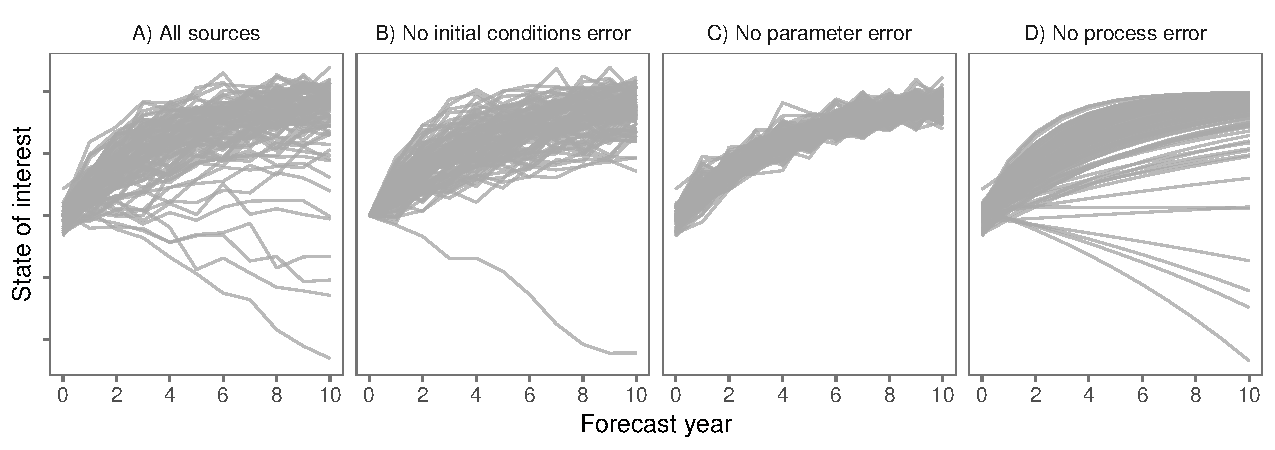
\includegraphics{../figures/forecast_uncertainty_example.pdf}
\caption{Example of forecast uncertainty with different sources of error
set to zero. Each line represents one realization, out of 200, from an
order-one autoregressive model (AR1 process). Contrary to the analytical
expression (Eq. 2), initial conditions uncertainty and parameter
uncertainty clearly interact. The spread of lines in (A) is not wholly
because of initial conditions uncertainty (B) or parameter uncertainty
(C), it is their combined influence that causes the spread of
realizations in (A). At least in this example, process error (D) does
appear to be independent, but we used a small value of process error to
highlight other interactions. Source code:
\texttt{generate\_forecast\_fxns.R}.}
\end{figure}

\hypertarget{a-brief-history-of-partioning-forecast-uncertainty}{%
\section{A Brief History of Partioning Forecast
Uncertainty}\label{a-brief-history-of-partioning-forecast-uncertainty}}

\hypertarget{weather-forecasting}{%
\subsection{Weather forecasting}\label{weather-forecasting}}

Chaos.

\hypertarget{earth-system-models}{%
\subsection{Earth system models}\label{earth-system-models}}

Carbon.

\hypertarget{dynamical-models}{%
\subsection{Dynamical models}\label{dynamical-models}}

Lotka-Volterra.

\hypertarget{a-simulation-based-approach-for-partitioning-forecast-uncertainty}{%
\section{A Simulation-Based Approach for Partitioning Forecast
Uncertainty}\label{a-simulation-based-approach-for-partitioning-forecast-uncertainty}}

Analytical expressions of forecast uncertainty must rely on simplifying
assumptions. Two important assumptions are (1) that different sources of
uncertainty do not interact and (2) that the system of equations is
linear. These analytical expressions are important for guiding our
intuition, but these strict assumptions limit our ability to partition
forecast uncertainty in practice. Thus, we present a simulation approach
that is entirely model-based and requires no assumptions, other than
those embedded in the model itself. We are building on the ideas put
forth by Dietze (2017), who suggested a simulation approach for
quantifying the terms in Eq. 2. Here we test the general idea using
simulated data and extend the approach to consider interactions among
sources of uncertainty.

As a starting point, consider a generic Bayesian state-space model

\begin{align}
\textbf{Data Model:} \quad y_t &\sim \left[y_t \;|\; z_t, \sigma^2_{\text{o}}\right], &t = 1,\dots,T, \\
\textbf{Process Models:} \quad z_t &\sim \left[z_t \;|\; \mu_t, \sigma^2_{\text{p}}\right],  \\
\mu_t &= g \left(z_{t-1},\textbf{x}'_t, \bm{\uptheta} \right), &t = 2,\dots,T, \\
\textbf{Parameter Models:} \quad \bm{\upphi} &\sim \left[\bm{\uptheta},\sigma^2_{\text{p}},\sigma^2_{\text{o}},z_{t=1} \right],
\end{align}

\noindent{}where \(y_t\) is the observed state at time \emph{t}, \(z_t\)
is the latent state at time \emph{t}, \(\mu_t\) is the determinstic
prediction of \emph{z} at time \emph{t} from the process model \emph{g},
which is a function of \emph{z} at time \emph{t-1}, a vector of
covariates (\textbf{x}) at time \emph{t}, and a set of unknown
parameters, \(\bm{\uptheta}\). \(\sigma^2_{\text{o}}\) is observation
error and \(\sigma^2_{\text{p}}\) is process error. The notation
\(\left[a \;|\; b, c\right]\) reads, ``the probability of \emph{a} given
\emph{b} and \emph{c}'' (Gelfand and Smith 1990), and \(\bm{\upphi}\)
refers to the prior probability distributions for all unknown parameters
and the initial conditions for the latent state, \(z_{t=1}\).

For our purposes, we are interested in the probability distributions of
the true state \textbf{z} at future points in time, conditional on
previous observations (\textbf{y}). This is referred to as the forecast
distribution or the predictive process distribution (Hobbs and Hooten
2015 pp. 199--200), which, for one time step ahead of the final
observation (\(T+1\)), is defined as

\begin{equation}
\begin{gathered}
\left[z_{T+1} | y_1,\dots,y_T \right] = \int \int \dots \int \left[z_{T+1} | z_T,\bm{\uptheta}, \sigma^2_{\text{p}} \right] \\ \times \left[z_1,\dots,z_T,\bm{\uptheta}, \sigma^2_{\text{p}} | y_1,\dots,y_T \right] d\bm{\uptheta} d\sigma^2_{\text{p}} dz_1 \dots dz_T.
\end{gathered}
\end{equation}

This type of model is easily fit using Bayesian methods and Markov chain
Monte carlo (MCMC) algorithms. The posterior distribution of all
unkowns, including states and parameters, is estimated over \emph{K}
MCMC iterations.

\begin{figure}
\centering
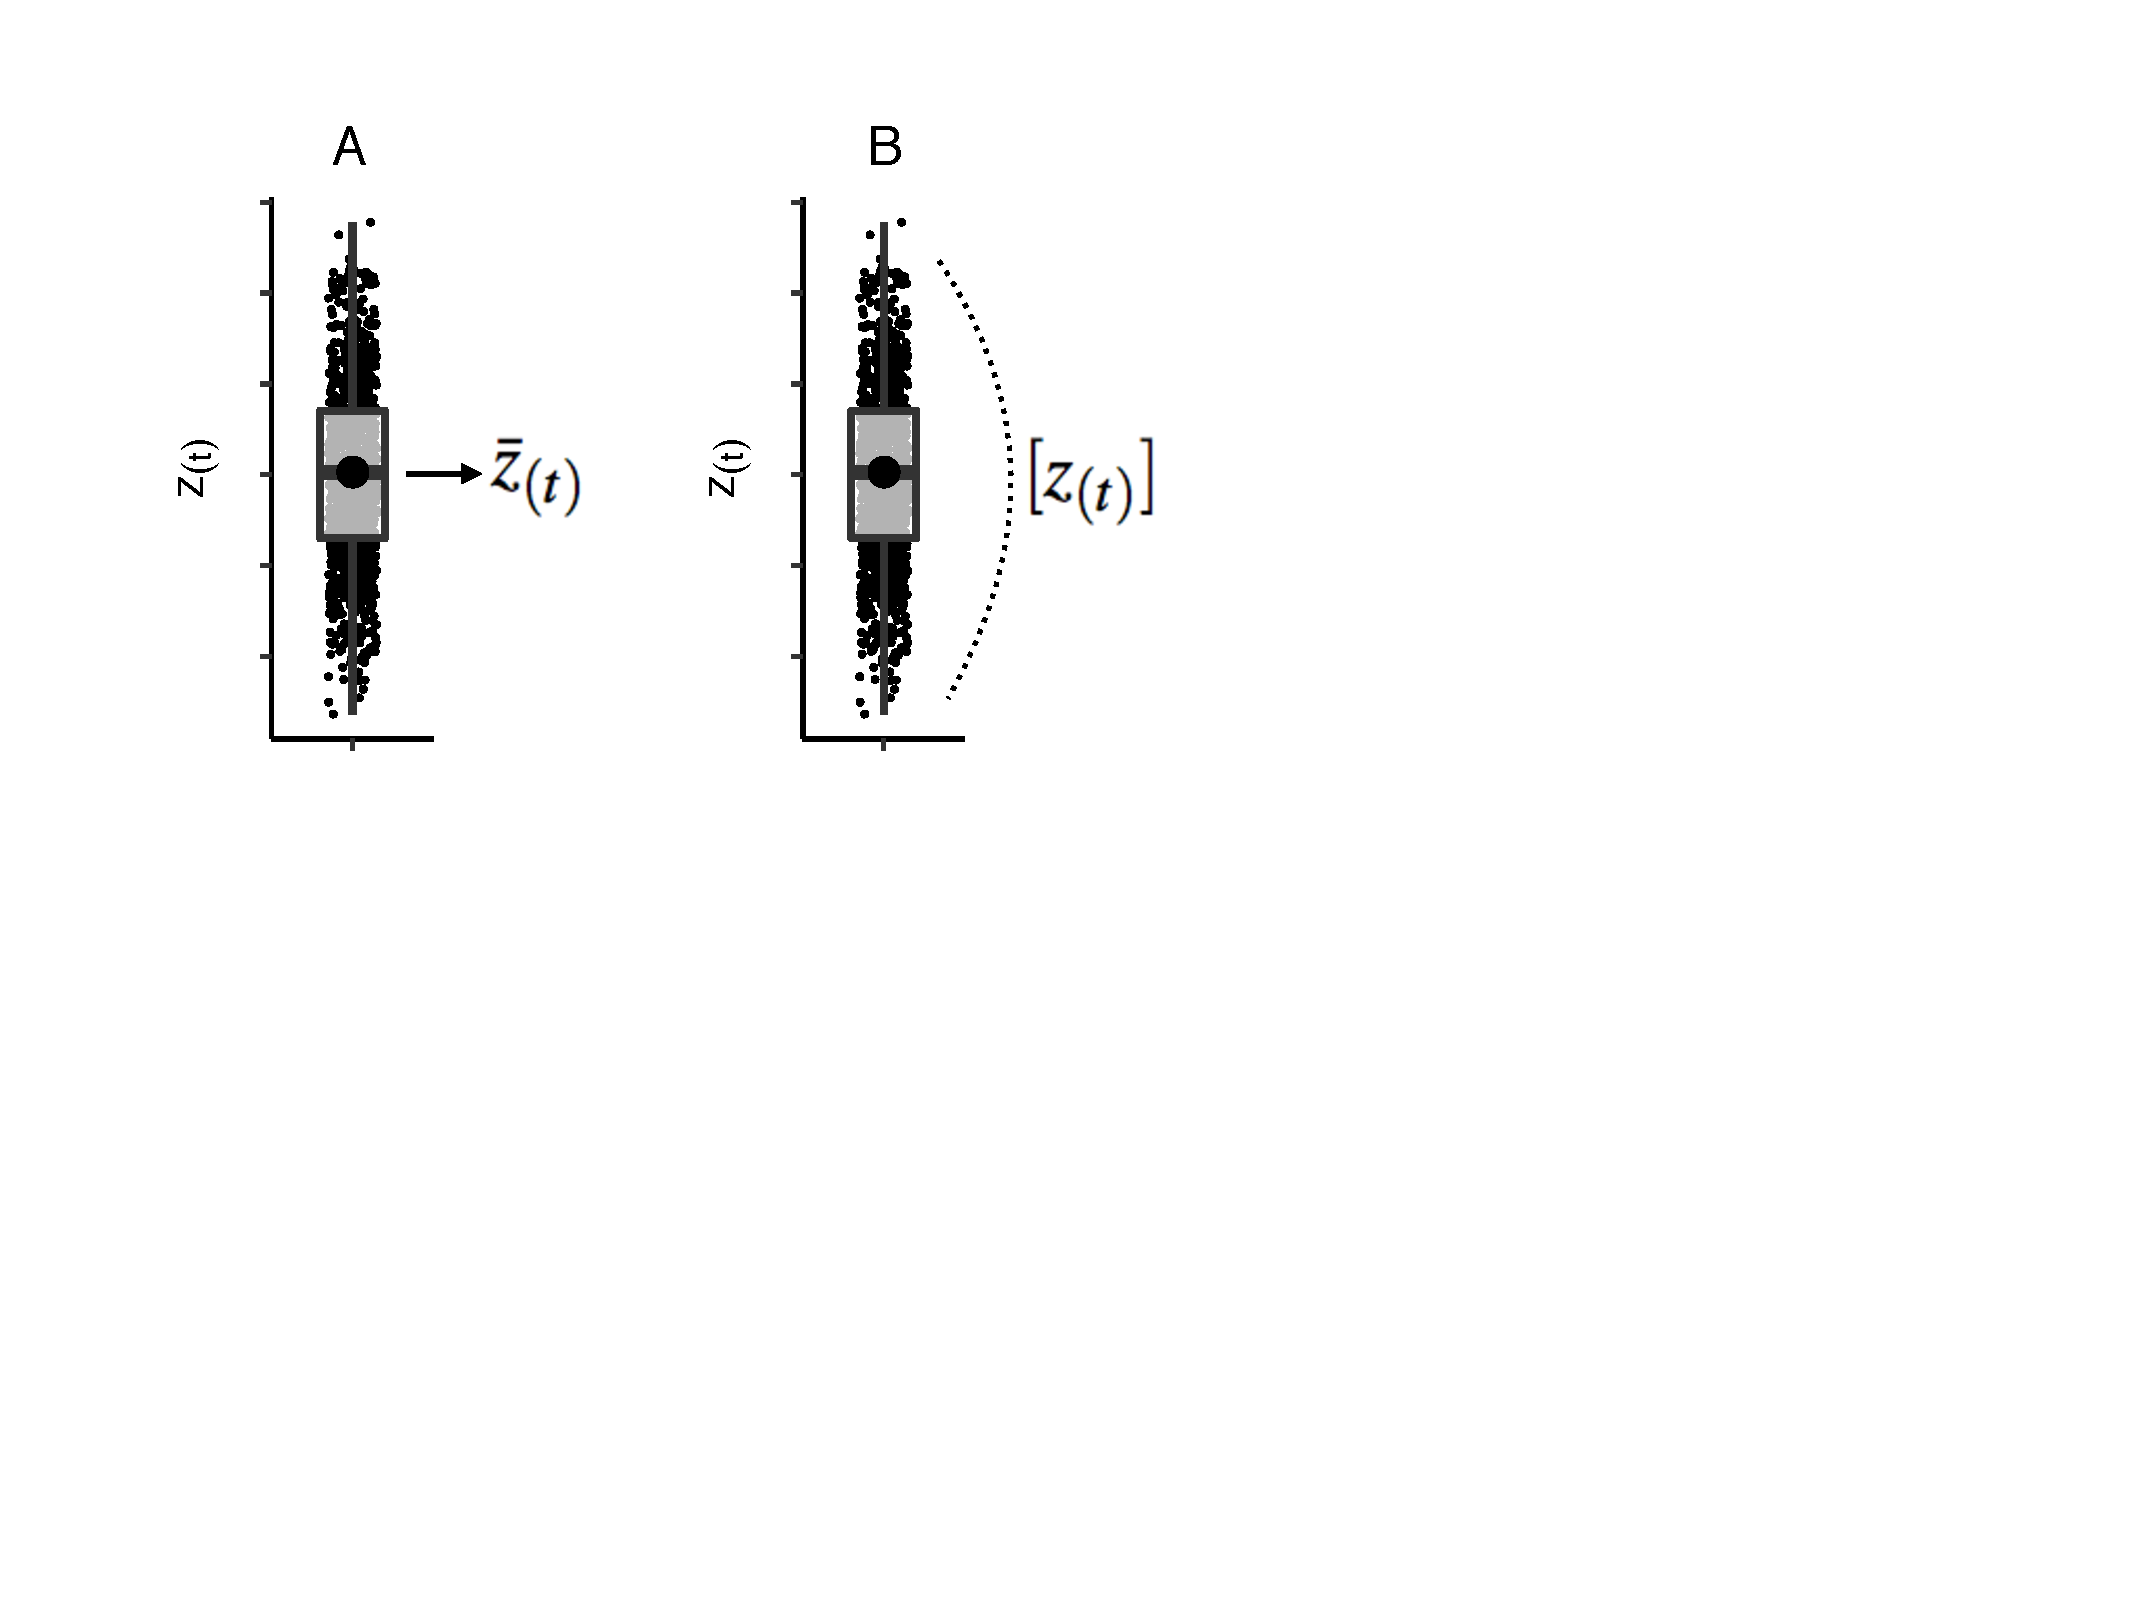
\includegraphics[width=\textwidth,height=2in]{../figures/init_cond_example.pdf}
\caption{Forecasts can be made using (A) a point estimate of the median
of the latent state \emph{z}, \(\bar{z}_{(t)}\), as a starting value or
(B) using the full distribution of \emph{z}, \([z_{(t)}]\). In both
panels, the small points are the estimates of \emph{z} at time \emph{t}
from each of 1000 MCMC iterations, the boxplots show the distribution,
and the large point shows the median. The scenario in A represents the
case where initial conditions uncertainty is set to zero. Comparing the
variance of forecasts made under scenarios A and B allows us to quantify
the amount of uncertainty attributable to initial conditions.}
\end{figure}

\hypertarget{application-yellowstone-bison-population}{%
\section{Application: Yellowstone Bison
Population}\label{application-yellowstone-bison-population}}

\hypertarget{references}{%
\section*{References}\label{references}}
\addcontentsline{toc}{section}{References}

\hypertarget{refs}{}
\leavevmode\hypertarget{ref-Bauer2015}{}%
Bauer, P., A. Thorpe, and G. Brunet. 2015. The quiet revolution of
numerical weather prediction. Nature 525:47--55.

\leavevmode\hypertarget{ref-Cariboni2007}{}%
Cariboni, J., D. Gatelli, R. Liska, and A. Saltelli. 2007. The role of
sensitivity analysis in ecological modelling. Ecological Modelling
203:167--182.

\leavevmode\hypertarget{ref-Clark2001}{}%
Clark, J. S., S. R. Carpenter, M. Barber, S. Collins, A. Dobson, J. A.
Foley, D. M. Lodge, M. Pascual, R. Pielke, W. Pizer, C. Pringle, W. V.
Reid, K. A. Rose, O. Sala, W. H. Schlesinger, D. H. Wall, and D. Wear.
2001. Ecological forecasts: an emerging imperative. Science
293:657--660.

\leavevmode\hypertarget{ref-Dietze2017a}{}%
Dietze, M. C. 2017. Prediction in ecology: A first-principles framework.
Ecological Applications 27:2048--2060.

\leavevmode\hypertarget{ref-Dietze2018}{}%
Dietze, M. C., A. Fox, L. M. Beck-Johnson, J. L. Betancourt, M. B.
Hooten, C. S. Jarnevich, T. H. Keitt, M. A. Kenney, C. M. Laney, L. G.
Larsen, H. W. Loescher, C. K. Lunch, B. C. Pijanowski, J. T. Randerson,
E. K. Read, A. T. Tredennick, R. Vargas, K. C. Weathers, and E. P.
White. 2018. Iterative near-term ecological forecasting: Needs,
opportunities, and challenges. Proceedings of the National Academy of
Sciences 115:1424--1432.

\leavevmode\hypertarget{ref-Gelfand1990}{}%
Gelfand, A. E., and A. F. Smith. 1990. Sampling-based approaches to
calculating marginal densities. Journal of the American Statistical
Association 85:398--409.

\leavevmode\hypertarget{ref-Hobbs2015}{}%
Hobbs, N. T., and M. B. Hooten. 2015. Bayesian Models: A Statistical
Primer for Ecologists. Princeton University Press, Princeton.

\leavevmode\hypertarget{ref-Sobol1993}{}%
Sobol', I. 1993. Sensitivity Estimates for Nonlinear Mathematical
Models.

\leavevmode\hypertarget{ref-Steffen2015}{}%
Steffen, W., K. Richardson, J. Rockström, S. Cornell, I. Fetzer, E.
Bennett, R. Biggs, and S. Carpenter. 2015. Planetary boundaries: Guiding
human development on a changing planet. Science 348:1217.


\end{document}
